\begin{capitulo}{Conceitos} \label{cap:concepts}


\paragrafo{Este capítulo tem como objetivo apresentar os conceitos provenientes dos livros e que serão utilizados na aplicação Web deste trabalho. }

\begin{secao}{Clean Architecture} \label{sec:carch}

\paragrafo{O livro Arquitetura Limpa, de Robert C. Martin, aborda vários conceitos importantíssimos referentes a arquitetura e facilidade de manutenção de sistemas. Neste trabalho será descrito apenas o que foi de fato implementado no sistema, sendo assim, os Princípios de Design (SOLID) e o próprio conceito de Arquitetura Limpa }

\begin{subsecao}{Arquitetura} \label{subsec:arquitetura}
  \paragrafo{Segundo Robert C. Martin, "Todo sistema de software fornece dois valores diferentes para os stakeholders: comportamento e estrutura. Desenvolvedores de software são responsáveis por garantir que ambos esses valores permaneçam altos". \cite[p.14]{clean_arch}}
  \paragrafo{O comportamento se trata da própria funcionalidade do sistema, ou seja, como o sistema se comporta de forma a economizar ou gerar dinheiro para os stakeholders. Se esse sistema para de funcionar ou necessita de uma manutenção, o desenvolvedor cria mais código a fim de tratar os problemas levantados.}
  \paragrafo{A estrutura, ou como iremos tratar nesse trabalho, a Arquitetura, se trata da forma que essas funcionalidades são desenvolvidas e o quão fácil é mudar esse sistema. Assim, quando os stakeholders decidem mudar o curso do projeto, a implementação dessa mudança não deveria ser mais díficil de ser realizada do que o próprio escopo da mudança.}
  \paragrafo{O problema principal que o autor levanta ao escrever o livro se trata de tanto desenvolvedores quanto gerentes de negócio priorizarem massivamente o primeiro, ignorando parcial ou totalmente o segundo valor que o software tem a oferecer. O autor argumenta, analisando as situações extremas:}
  
  \begin{lista}
   \itemlista{"Se você me der um programa que funcione perfeitamente, mas seja impossível de mudar, então ele não funcionará quando as exigências mudarem e eu não serei capaz de fazê-lo funcionar. Portanto, o programa será inútil".}
   \itemlista{"Se você me der um programa que não funcione, mas seja fácil de mudar, então eu posso fazê-lo funcionar, e posso mantê-lo funcionando à medida que as exigências mudarem. Portanto, o programa permanecerá continuamente útil".}\cite[p.16]{clean_arch}
    \vspace{0.6cm}
  \end{lista}

  \paragrafo{Concluindo este tema, o objetivo de termos uma boa arquitetura de software pode ser descrito, conforme diz o próprio autor, de forma utópica, da seguinte forma: "O objetivo da arquitetura de software é minimizar os recursos humanos necessários para construir e manter um determinado sistema". \cite[p.5]{clean_arch}}

\end{subsecao}

\begin{subsecao}{SOLID} \label{subsec:solid}
  \paragrafo{Os princípios SOLID, em resumo, se tratam de regras de organização de funções e estruturas de dados em agrupamentos. O principal objetivo de sua aplicação está em criar software que seja de fácil entendimento, manutenção e reaproveitamento.}
  \paragrafo{Também proposto por Robert C. Martin, SOLID é um acrônimo para outras siglas:}
  \begin{lista}
   \itemlista{Princípio da Responsabilidade Única (\emph{Single Responsiblity Principle})}
   \itemlista{Princípio do Aberto/Fechado (\emph{Open-Closed Principle})}
   \itemlista{Princípio de Substituição de Liskov (\emph{Liskov Substitution Principle})}
   \itemlista{Princípio da Segregação de Interface (\emph{Interface Segregation Principle})}
   \itemlista{Princípio da Inversão de Dependência (\emph{Dependency Inversion Principle})}
    \vspace{0.6cm}
  \end{lista}
  \paragrafo{Definindo os príncipios, bem resumidamente, teríamos:}
  \begin{lista}
   \itemlista{\acs{SRP} - Cada módulo de software deve ser estruturado de forma que haja uma, e apenas uma, razão para mudar.}
   \itemlista{\acs{OCP} - Para que o software seja fácil de mudar, deve ser projetado para garantir que o mesmo está aberto à adição, mas fechado para alteração.}
   \itemlista{\acs{LSP} - Criando um sistema a partir de partes trocáveis entre si, estas partes devem firmar um contrato que permita que uma seja substituída pela outra.}
   \itemlista{\acs{ISP} - Deve-se evitar que o software dependa de métodos que não usa.}
   \itemlista{\acs{DIP} - Código de nível mais alto (Próximo às regras de negócio) não deve depender de código de nível mais baixo (detalhes de implementação, \emph{frameworks}, banco de dados).}
    \vspace{0.6cm}
  \end{lista}
  \paragrafo{Os exemplos da implementação desses princípios serão fornecidos posteriormente neste mesmo trabalho, no Capítulo 4.}
\end{subsecao}

\begin{subsecao}{Arquitetura Limpa} \label{subsec:carch}
\paragrafo{Robert C. Martin menciona que toda boa arquitetura teria um objetivo principal, que é a Separação de Preocupações (\emph{Separation of Concerns}). Esta consiste em dividir, em níveis, todo o código desenvolvido. Esses níveis podem ser representados como circulos circuncêntricos, de forma que as camadas de nível mais alto do código estejam mais ao centro do círculo, tal como a Figura \ref{fig:carch}.}
\begin{figure}[h!]
  \centering
  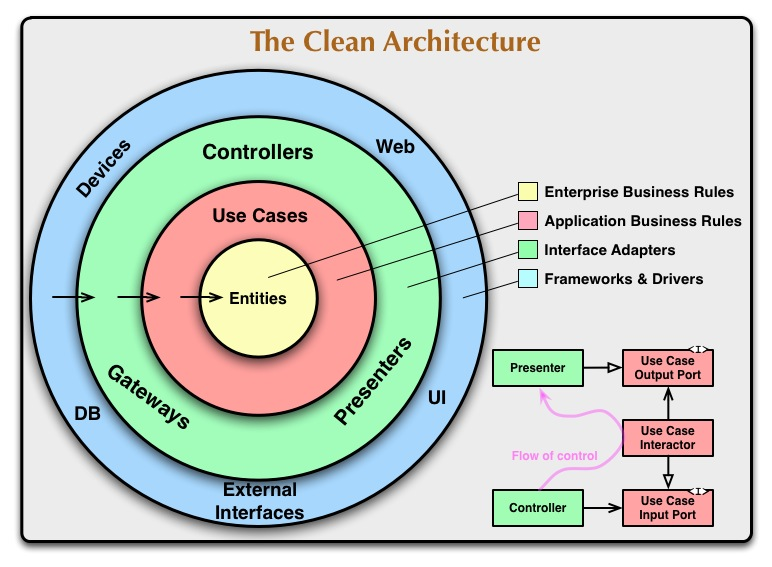
\includegraphics[scale=0.5]{CleanArchitecture}
  \caption{A arquitetura limpa}
  \label{fig:carch}
\end{figure}
\paragrafo{A seguir, será detalhado do que cada nível se trata, e para ajudar nesse detalhamento, usaremos como exemplo um sistema de gerenciamento de usuários.}
\paragrafo{Regras de Negócio de Empresa (\emph{Enterprise Business Rules}), ou as Entidades, são objetos com suas próprias funções ou estruturas de dados que possam ser utilizadas por várias aplicações diferentes numa mesma empresa. No contexto desse trabalho e na maioria das aplicações web, as entidades serão as tabelas do banco de dados, devido a sua grande tendência de reutilização em diferentes partes de um mesmo sistema. No exemplo proposto, a entidade seria uma tabela de usuários com os atributos do mesmo, como o nome, endereço, login e senha.}
\paragrafo{Regras de Negócio da Aplicação (\emph{Application Business Rules}), ou os Casos de Uso, são todos os fluxos especificos de uma aplicação. Essas regras de negócio utilizam-se manipulam as Entidades a fim de processar o que lhes for pedido. No exemplo proposto, os casos de uso seriam os algoritmos de cadastro, autenticação, consulta, atualização, remoção e outras tarefas referentes à tabela previamente apresentada.}
\paragrafo{Os Adaptadores de Interface (\emph{Interface Adapters}) tem como propósito converter os dados entre os níveis vizinhos de uma forma que seja conveniente para todos os envolvidos. Um exemplo de adaptador no sistema pode ser uma classe responsável por tratar as requisições recebidas pelos frameworks a fim de executar os casos de uso para gerenciar os usuários.}
\paragrafo{Por fim, os Frameworks e Drivers são geralmente, no contexto de desenvolvimento web, as ferramentas usadas para acesso a banco de dados e web. Por serem ferramentas já prontas, geralmente só é desenvolvido nessa camada a comunicação com os níveis mais internos.}
\paragrafo{O importante sobre essa divisão em camadas é garantir que mudanças nas camadas externas não afetem as camadas internas, possibilitando apenas que as mudanças nas camadas internas tragam consequências às camadas externas. Esse seria o conceito de Regra da Dependência, que consiste em garantir que as dependências do código partam apenas de fora para dentro do círculo.}
\paragrafo{Em resumo, um sistema que separa suas preocupações e que segue a Regra da Dependência tendem ter uma arquitetura limpa, com módulos de lógica de negócios testáveis, independentes de frameworks, UI, banco de dados ou qualquer agência externa.}
\end{subsecao}
\end{secao}

\begin{secao}{Design Patterns} \label{sec:patterns}

  \paragrafo{Como alguns princípios vistos na seção de Clean Architecture, os Design Patterns tem como principal função garantir a reusabilidade do código com baixo acoplamento. De fato, a proposta principal do livro está em ser um catálogo de soluções para problemas de sistemas orientados a objetos.}
  \paragrafo{No total, são 23 padrões de projetos diferentes, subdividos em 3 tipos: Padrões de Criação, Padrões Comportamentais e Padrões Estruturais:}
  
  \paragrafo{Padrões de Criação}
  \begin{lista}
   \itemlista{Abstract Factory}
   \itemlista{Builder}
   \itemlista{Factory Method}
   \itemlista{Prototype}
   \itemlista{Singleton}
  \end{lista}

  \paragrafo{Padrões Estruturais}
  \begin{lista}
    \itemlista{Adapter}
    \itemlista{Bridge}
    \itemlista{Composite}
    \itemlista{Decorator}
    \itemlista{Facade}
    \itemlista{Flyweight}
    \itemlista{Proxy}
  \end{lista}
  
  \paragrafo{Padrões Comportamentais}
  \begin{lista}
    \itemlista{Chain of Responsiblity}
    \itemlista{Command}
    \itemlista{Interpreter}
    \itemlista{Iterator}
    \itemlista{Mediator}
    \itemlista{Memento}
    \itemlista{Observer}
    \itemlista{State}
    \itemlista{Strategy}
    \itemlista{Template Method}
    \itemlista{Visitor}
  \end{lista}
  
  \paragrafo{Não faz parte da proposta desse trabalho usar cada um dos padrões supracitados. A proposta está em identificar as oportunidades de aplicação durante as etapas de desenvolvimento. Como o sistema, até o atual momento, não está pronto, será necessário revisitar esse capítulo posteriormente listando e explicando cada padrão usado na aplicação web.}
\end{secao}

\end{capitulo}